\subsection{HMBC low-pass J-filter}
\label{subsec:poise__hmbc}

In this and the remaining examples, we look at optimisations involving \textit{multiple parameters}, one of the key strengths of POISE.
Grid searches are extremely ineffective for this purpose, as the number of FEs required scales exponentially with the number of parameters; human trial-and-error can also be very difficult as parameters may be tightly \textit{coupled}, meaning that the optimum cannot simply be found by optimising one parameter at a time.
In contrast, the optimisation algorithms used in POISE make no assumption about the relationship between the two parameters.
Furthermore, since only local minima are sought, the time required for convergence scales approximately linearly with the number of parameters, at least in the regimes which I have tested.%
\footnote{I am not actually aware of any \textit{theoretical} results which show how the number of function evaluations scales with the number of parameters in an optimisation; I suspect the answer depends on the exact problem being solved.}

\begin{figure}[htb]
    \centering
    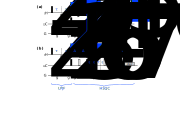
\includegraphics[]{pp/poise/hmbc.png}%
    {\phantomsubcaption\label{fig:poise_hmbc_pulseq_hmbc}}%
    {\phantomsubcaption\label{fig:poise_hmbc_pulseq_hsqc}}%
    \caption[Pulse sequences used for HMBC optimisation]{
        \textbf{(\subref*{fig:poise_hmbc_pulseq_hmbc})} Standard 2D HMBC pulse sequence with a second-order LPJF.
        \textbf{(\subref*{fig:poise_hmbc_pulseq_hsqc})} 1D LPJF--HSQC pulse sequence used in the POISE optimisation.
        In practice, only the first increment of this experiment was recorded.
        Delays are set as follows: $\Delta = 1 / (4 \cdot \oneJ{CH}); \Delta_\text{LR} = 1 / (2 \cdot \nJ{CH})$; $\tau$ is as short as possible (several microseconds); and $\tau_1$ and $\tau_2$ are as described in the text.
        Phase cycling is performed with $\phi_1 = \phirec = (x, -x)$, and $\phi_2 = (x, x, -x, -x)$.
        Gradient amplitudes are: $(g_1, g_2, g_3) = (15\%, -10\%, -5\%)$ for the LPJF, $(g_4, g_5) = (80\%, -47.85\%)$ (or vice versa) for EA selection in the HMBC experiment\autocite{Cicero2001JMR}, and $(g_6, g_7) = (70\%, \pm 35.21\%)$ for EA selection in the LPJF--HSQC experiment.
    }
    \label{fig:poise_hmbc_pulseq}
\end{figure}

In the simplest example of a multiple-parameter optimisation, I use POISE to search for the best delays in the low-pass J-filter (LPJF) of a HMBC experiment (\cref{fig:poise_hmbc_pulseq_hmbc}).
Specifically, a second-order LPJF is used, which has the form $\tau_1$--\ang{90}(\carbon{})--$\tau_2$--\ang{90}(\carbon{}).
The role of the LPJF is to destroy \magn{C} magnetisation at the start of the HMBC, which would otherwise generate one-bond artefacts in the resulting spectrum.
Assuming that the $\oneJ{CH}$ values span a range of $\Jmin$ to $\Jmax$, S{\o}rensen and coworkers have provided `theoretical' best values for the delays:\autocite{Nielsen1986JMR,Meissner2000MRC}
\begin{align}
    \tau_1 &= \frac{1}{2} [\Jmin + 0.146(\Jmax - \Jmin)]^{-1}; \label{eq:hmbc_lpjf_theoretical_min} \\
    \tau_2 &= \frac{1}{2} [\Jmax - 0.146(\Jmax - \Jmin)]^{-1}. \label{eq:hmbc_lpjf_theoretical_max}
\end{align}
In practice, the TopSpin standard library HMBC sequence (\texttt{hmbcetgpl2nd}) uses delays of
\begin{equation}
    \tau_1 = \frac{1}{2\Jmin}; \quad \tau_2 = \frac{1}{2\Jmax}. \label{eq:hmbc_lpjf_bruker}
\end{equation}
In either case, though, these delays neglect the actual \textit{distribution} of $\oneJ{CH}$: if many of the couplings are clustered around one particular value, then adjusting the delays to better suppress these values will yield better results.
(Since $\oneJ{CH}$ roughly correlates with the hybridisation of the \carbon{} atom,\autocite{Krivdin2018PNMRS} this can easily happen, for example, if the molecule is predominantly aliphatic or predominantly aromatic.)


\subsubsection{Optimisation setup}

In order for the optimisation routine to minimise the artefacts, it must first have a cost function which can measure the extent of these artefacts.
Given a full 2D HMBC spectrum, it is very difficult to discern which of the peaks are indeed artefacts (this is exactly why it is worthwhile to suppress them).
However, by using a specially designed LPJF--HSQC experiment (\cref{fig:poise_hmbc_pulseq_hsqc}), the artefacts can be isolated without any of the HMBC signals appearing:
this works because any \magn{C} magnetisation which is \textit{not} destroyed by the LPJF will be sampled in the HSQC segment which follows.
Although the LPJF--HSQC can in principle be recorded as a full 2D experiment, to save time, I chose to only record the first increment as a 1D experiment.
\carbon{} decoupling during acquisition is not mandatory, but the boost in SNR obtained through decoupling shortens the time needed for optimisation, and also reduces noise in the cost function.

We could directly perform an optimisation on the two delays $\tau_1$ and $\tau_2$.
However, for simplicity, I chose to reuse the definitions of $\tau_1$ and $\tau_2$ in the Bruker library sequence (\cref{eq:hmbc_lpjf_bruker}) and instead optimise the parameters $\Jmin' = 1/(2\tau_1)$ and $\Jmax' = 1/(2\tau_2)$: these are represented in the pulse sequence as \texttt{CNST25} and \texttt{CNST26} respectively.%
\footnote{Prime symbols are used here because $\Jmin$ and $\Jmax$ are \textit{physical constants} which depend on the sample being studied, whereas $\Jmin'$ and $\Jmax'$ are \textit{parameters} which can be chosen to have any value.} 
Both parameters were constrained to lie between 100 and \qty{200}{\Hz}, with a tolerance of \qty{3}{\Hz}.
To match the magnitude-mode processing typically used for 2D HMBC experiments, the acquisition AU programme was modified to also process the LPJF--HSQC spectrum in magnitude mode.
The integral of the entire spectrum can therefore be used as the desired cost function for the POISE optimisation.
More specifically, I chose to use a sum of squares:
\begin{equation}
    \label{eq:sos_cost_function}
    f_{\symup{sos}} = \sum_i S_i^2,
\end{equation}
which has the effect of penalising intense artefacts more strongly.


\subsubsection{Optimisation results}

In previous sections, I have quoted ranges for the optima found in an effort to show that the optimisation results were reproducible.
In multiple-parameter optimisations, it is no longer appropriate to report separate ranges for both parameters, since the parameters are in general \textit{interdependent}, in that the spread of values obtained for the first parameter depends on the value obtained for the second, and vice versa.
I therefore only provide ranges for the number of FEs, as well as the time taken.
As for optima found, I will quote only the \textit{best} of these, as measured by the reduction in the cost function.
These optima should therefore not be viewed as a complete summary of the five different runs, but rather as an \textit{example} of the improvement which may be obtained through POISE.

\begin{table}[htb]
    \hbadness=10000
    \centering
    \begin{tabular}{ccccccc}
        \toprule
              &           & \multicolumn{3}{c}{Best optimum found} & \multicolumn{2}{c}{Aggregated results} \\
        \cmidrule(lr){3-5} \cmidrule(lr){6-7}
        Entry & Algorithm & $\Jmin'$ & $\Jmax'$ & $\fsos / 10^7$ & FEs & Time taken (\unit{\s}) \\
        \midrule
        1     & NM        & 143.07 & 185.71                 & 8.65 & 20--24 & 358--430 \\
        2     & MDS       & 141.73 & 185.82                 & 8.36 & 18     & 321--323 \\
        3     & BOBYQA    & 133.38 & 155.03                 & 6.42 & 14--17 & 251--304 \\
        \bottomrule
    \end{tabular}
    \caption[HMBC low-pass J-filter optimisations]{
        Results of HMBC POISE optimisations.
        For each optimisation algorithm, the best optimum found is reported along with the value of the cost function $\fsos$ (a lower value represents a better optimum).
        The number of FEs, as well as the time taken, is still reported as a range over the five optimisation runs performed per algorithm.
        The POISE routine used here is: \mintinline[breaklines]{json}{{"name": "lpjf", "pars": ["cnst25", "cnst26"], "lb": [100.0, 100.0], "ub": [200.0, 200.0], "init": [120.0, 180.0], "tol": [3.0, 3.0], "cf": "zerorealint_squared", "au": "poise_1d_mc"}}.
        \datacode{7Z-210814}
    }
    \label{tbl:poise_hmbc}
\end{table}

\begin{figure}[htb]
    \centering
    \includegraphics[]{poise/hmbc_scan.png}%
    \caption[Reference grid search for HMBC optimisation]{
        Reference grid search for HMBC optimisation.
        Darker regions correspond to lower cost function values, i.e.\ better spectra.
        The results of the 15 optimisations (5 per algorithm) are plotted on the same axes.
        Note that the cost functions here are rather larger than in \cref{tbl:poise_hmbc}: this is solely because a different receiver gain was used.
        \datacode{7Z-210814}
    }
    \label{fig:poise_hmbc_scan}
\end{figure}

Interestingly, BOBYQA finds an optimum which is different from---and substantially better than---the other two algorithms.
As mentioned previously, it is not generally possible to predict which optimum an algorithm will converge to, and this is complicated even further by the presence of noise, which imparts some stochastic character to the optimisation.
Nevertheless, a closer inspection of the other optimisation runs actually shows that the better performance of BOBYQA on this problem is reproducible: the optima found from each of the five rounds, as well as a reference grid search, are plotted in \cref{fig:poise_hmbc_scan}.
It appears that the simplex-based methods get stuck in a suboptimal region, whereas BOBYQA is usually able to move leftwards and downwards into a more productive region.
However, the exact reasons for this remain unclear.
Also, BOBYQA does not always outperform NM and MDS in the other optimisations in this chapter (this is possibly a manifestation of the `no free lunch theorem'\autocite{Wolpert1997IEEETEC}, which states that when averaged over all problems, no optimisation algorithm strictly outperforms another).

\begin{figure}[htb]
    \centering
    \includegraphics[]{poise/hmbc_spec.png}%
    {\phantomsubcaption\label{fig:poise_hmbc_spec_unopt2}}%
    {\phantomsubcaption\label{fig:poise_hmbc_spec_opt2}}%
    {\phantomsubcaption\label{fig:poise_hmbc_spec_3}}%
    \caption[HMBC spectra before and after optimisation]{
        \textbf{(\subref*{fig:poise_hmbc_spec_unopt2})} HMBC spectrum with `compromise' values of 120 and \qty{180}{\Hz} for $\Jmin'$ and $\Jmax'$ respectively in the second-order LPJF.
        The one-bond artefacts are highlighted in red boxes.
        \textbf{(\subref*{fig:poise_hmbc_spec_opt2})} HMBC spectrum with optimised second-order LPJF delays.
        \textbf{(\subref*{fig:poise_hmbc_spec_3})} HMBC spectrum with third-order LPJF.
        \datacode{7Z-210814}
    }
    \label{fig:poise_hmbc_spec}
\end{figure}

In any case, when the best of these optimised values (i.e.\ entry 3 in \cref{tbl:poise_hmbc}) were used to run a standard 2D HMBC, a significant reduction in one-bond artefacts was observed.
It should be emphasised that these optimised values were obtained in a matter of several minutes, which is far shorter than a typical HMBC experiment requires.
The performance of the optimised second-order LPJF (\cref{fig:poise_hmbc_spec_opt2}) was in fact almost comparable to that of a third-order LPJF (\cref{fig:poise_hmbc_spec_3}).
However, using a third-order LPJF risks suppressing some of the desired HMBC signal as well, so if all else is equal, the optimised second-order LPJF should be preferred.
In principle, the third-order LPJF itself can also be subjected to optimisation: this possibility was not explored in the present work, but would be easy to set up using the methods outlined in this section.


\subsubsection{Application to NOAH HMBC}

\begin{figure}[htb]
    \centering
    \includegraphics[]{pp/hmbc/noah_no90.png}%
    \caption[NOAH HMBC module]{
        NOAH HMBC module.
    }
    \label{fig:noah_hmbc_no90}
\end{figure}

In NOAH supersequences, the HMBC experiment (or `module') is typically modified by replacing the initial \ang{90} excitation pulse with a $zz$-filter (\cref{fig:noah_hmbc_no90}).\autocite{Kupce2018CC,Kupce2019JMR}
This causes the \magnnot{C} magnetisation used in the HMBC to be excited, but leaves \magn{C} magnetisation along the $+z$ axis so that it can be preserved for later modules in a supersequence.
In an ideal situation, this means that the one-bond artefacts in the HMBC should in fact be suppressed even without an LPJF.
However, significant one-bond artefacts are in fact still observed in NOAH HMBC spectra.
I therefore sought to apply the same optimisation routine to the $zz$-HMBC module to see whether this could be improved.


\begin{table}[htb]
    \hbadness=10000
    \centering
    \begin{tabular}{ccccccc}
        \toprule
              &           & \multicolumn{3}{c}{Best optimum found} & \multicolumn{2}{c}{Aggregated results} \\
        \cmidrule(lr){3-5} \cmidrule(lr){6-7}
        Entry & Algorithm & $\Jmin'$ & $\Jmax'$ & $\fsos / 10^9$ & FEs & Time taken (\unit{\s}) \\
        \midrule
        1     & NM        & 117.05 & 188.59                 & 5.37 & 25--29 & 451--523 \\
        2     & MDS       & 125.21 & 193.16                 & 5.35 & 14--17 & 249--310 \\
        3     & BOBYQA    & 119.49 & 182.74                 & 5.78 & 9--16  & 164--293 \\
        \bottomrule
    \end{tabular}
    \caption[NOAH HMBC low-pass J-filter optimisations]{
        Results of POISE optimisations on the LPJF in the NOAH HMBC module.
        All optimisation details are the same as in \cref{tbl:poise_hmbc}, except that the LPJF--HSQC pulse sequence used for the optimisation was modified accordingly to include a $zz$-filter.
        \datacode{7Z-210814}
    }
    \label{tbl:poise_hmbc_noah}
\end{table}

Unfortunately, the results here were far less impactful: generally, the optimisation converged to values very close to the initial starting point, and in some cases the behaviour of the optimised spectrum was even (very slightly) worse than the unoptimised spectrum.
(The deterioration is very marginal, and likely arises only due to noise in the cost function during the optimisation.)
This strongly suggests that the artefacts are not due to imperfect LPJF suppression, but instead stem from the $zz$-filter component of the sequence.
This was indeed verified experimentally: the addition of a \carbon{} \ang{90} pulse at the end of the $zz$-filter led to much better one-bond artefact suppression (\cref{fig:poise_hmbc_noah_spec_with90}; this strategy is further explained in \cref{subsec:noah__hmbc}).

\begin{figure}[htb]
    \centering
    \includegraphics[]{poise/hmbc_noah_spec.png}%
    {\phantomsubcaption\label{fig:poise_hmbc_noah_spec_unopt}}%
    {\phantomsubcaption\label{fig:poise_hmbc_noah_spec_opt}}%
    {\phantomsubcaption\label{fig:poise_hmbc_noah_spec_with90}}%
    \caption[NOAH HMBC spectra before and after optimisation]{
        \textbf{(\subref*{fig:poise_hmbc_noah_spec_unopt})} NOAH HMBC spectrum before POISE optimisation, using the default settings of 120 and \qty{180}{\Hz}.
        One-bond artefacts are highlighted in red boxes.
        \textbf{(\subref*{fig:poise_hmbc_noah_spec_opt})} NOAH HMBC spectrum after POISE `optimisation' (using $\Jmin' = \qty{125.2}{\Hz}$, $\Jmax' = \qty{193.2}{\Hz}$, as per entry 2 of \cref{tbl:poise_hmbc_noah}).
        \textbf{(\subref*{fig:poise_hmbc_noah_spec_with90})} NOAH HMBC spectrum with no POISE optimisation, but instead adding a \ang{90} \carbon{} pulse at the end of the $zz$-filter (see also \cref{subsec:noah__hmbc}).
        \datacode{7Z-210814}
    }
    \label{fig:poise_hmbc_noah_spec}
\end{figure}
